% Standalone figure: run make in this directory to build PDF and SVG.
\documentclass[11pt,tikz,border=0pt]{standalone}
\usepackage{fontspec}
\IfFontExistsTF{Helvetica Neue Light}{
  \setsansfont{Helvetica Neue Light}[BoldFont={Helvetica Neue Medium}]
  \newfontfamily\vnmedium{Helvetica Neue Medium}
}{
  \setsansfont{TeX Gyre Heros}
  \newcommand{\vnmedium}{\bfseries}
}
\renewcommand{\familydefault}{\sfdefault}
\usepackage{amsmath,amssymb,mathtools}
\usepackage{unicode-math}
\setmathfont{latinmodern-math.otf}
\usetikzlibrary{arrows.meta,calc,positioning}
\definecolor{vnslideink}{HTML}{333333}
\definecolor{vnslidebody}{HTML}{5E5E5E}
\definecolor{vnaccent}{HTML}{FF644E}
\definecolor{vnslidelink}{HTML}{579ACA}
\pagecolor{white}


\definecolor{treeAccent}{HTML}{EF4136}
\definecolor{treeGray}{HTML}{777777}
\definecolor{treeLeaf}{HTML}{E9E9E9}
\definecolor{treeGuide}{HTML}{D7D7D7}
\begin{document}
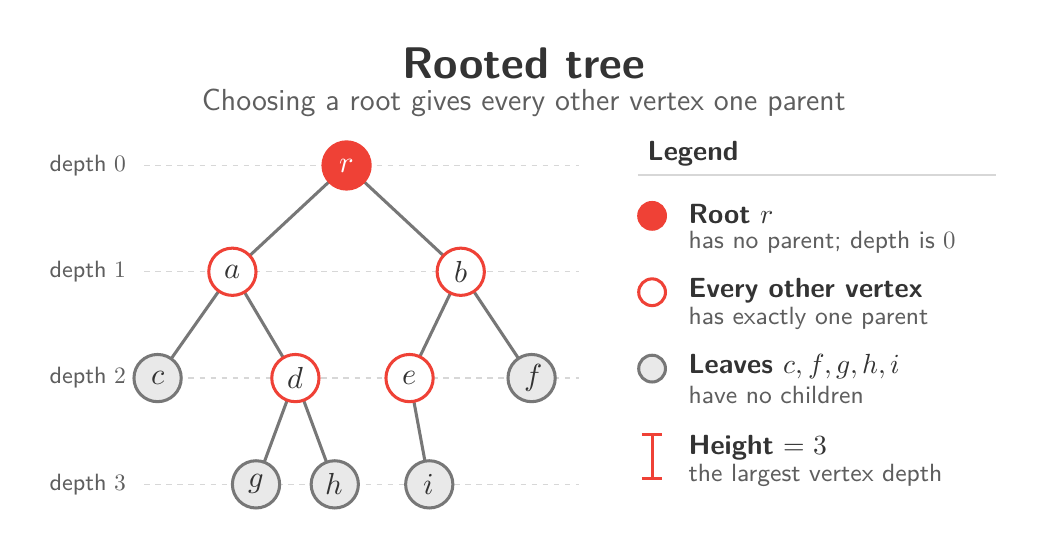
\begin{tikzpicture}[x=1cm,y=1cm,text=vnslideink,
  font=\sffamily\fontsize{11}{13}\selectfont,
  treevertex/.style={circle,minimum size=6mm,inner sep=0pt,line width=1.1pt},
  internal/.style={treevertex,draw=treeAccent,fill=white},
  root/.style={treevertex,draw=treeAccent,fill=treeAccent,text=white},
  leaf/.style={treevertex,draw=treeGray,fill=treeLeaf},
  legendheading/.style={anchor=west,font=\sffamily\bfseries\fontsize{10}{12}\selectfont},
  legenddetail/.style={anchor=west,text=vnslidebody,font=\sffamily\fontsize{9}{11}\selectfont}]
  \ifdefined\TreeGraphOmitHeading
    \fill[white] (-0.4,0.65) rectangle (12.2,5.7);
    \path[use as bounding box] (-0.4,0.65) rectangle (12.2,5.7);
  \else
    \fill[white] (-0.4,0.65) rectangle (12.2,6.95);
    \node[font=\sffamily\bfseries\fontsize{16}{19}\selectfont] at (5.9,6.5) {Rooted tree};
    \node[text=vnslidebody] at (5.9,5.99)
      {Choosing a root gives every other vertex one parent};
    \path[use as bounding box] (-0.4,0.65) rectangle (12.2,6.95);
  \fi

  % Depth guides remain behind the undirected edges and vertices.
  \foreach \depth/\y in {0/5.2,1/3.85,2/2.5,3/1.15} {
    \node[anchor=east,inner sep=0pt,text=vnslidebody,font=\sffamily\fontsize{8.5}{10}\selectfont]
      at (0.86,\y) {depth $\depth$};
    \draw[draw=treeGuide,line width=0.5pt,dash pattern=on 2pt off 2pt]
      (1.08,\y)--(6.6,\y);
  }
  \foreach \v/\x/\y in {r/3.65/5.2,a/2.2/3.85,b/5.1/3.85,c/1.25/2.5,d/3/2.5,e/4.45/2.5,f/6/2.5,g/2.5/1.15,h/3.5/1.15,i/4.7/1.15}
    {\coordinate (\v) at (\x,\y);}
  \foreach \u/\v in {r/a,r/b,a/c,a/d,b/e,b/f,d/g,d/h,e/i}
    {\draw[draw=treeGray,line width=1.1pt] (\u)--(\v);}
  \node[root] at (r) {$r$};
  \foreach \v in {a,b,d,e} {\node[internal] at (\v) {$\v$};}
  \foreach \v in {c,f,g,h,i} {\node[leaf] at (\v) {$\v$};}

  \node[anchor=west,font=\sffamily\bfseries] at (7.35,5.35) {Legend};
  \draw[draw=treeGuide,line width=0.5pt] (7.35,5.08)--(11.9,5.08);

  \node[root,minimum size=3.4mm] at (7.53,4.56) {};
  \node[legendheading] at (7.87,4.58) {Root $r$};
  \node[legenddetail] at (7.87,4.23) {has no parent; depth is $0$};

  \node[internal,minimum size=3.4mm] at (7.53,3.59) {};
  \node[legendheading] at (7.87,3.61) {Every other vertex};
  \node[legenddetail] at (7.87,3.26) {has exactly one parent};

  \node[leaf,minimum size=3.4mm] at (7.53,2.62) {};
  \node[legendheading] at (7.87,2.64) {Leaves $c,f,g,h,i$};
  \node[legenddetail] at (7.87,2.29) {have no children};

  \draw[draw=treeAccent,line width=1.1pt] (7.4,1.78)--(7.66,1.78)
    (7.53,1.78)--(7.53,1.23) (7.4,1.23)--(7.66,1.23);
  \node[legendheading] at (7.87,1.61) {Height $=3$};
  \node[legenddetail] at (7.87,1.26) {the largest vertex depth};
\end{tikzpicture}
\end{document}
